
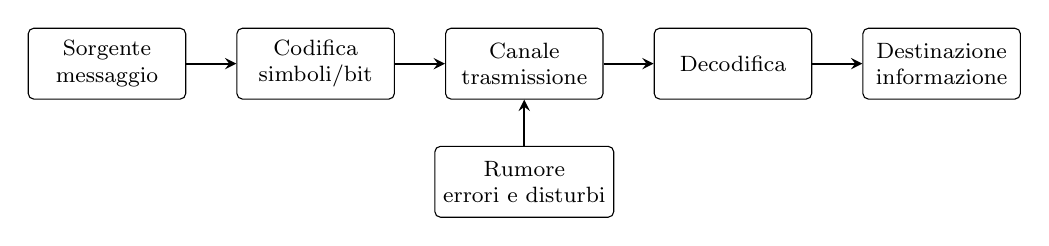
\begin{tikzpicture}[
  >=stealth,
  blocco/.style={
    draw,
    rounded corners=2pt,
    align=center,
    minimum width=2cm,
    minimum height=0.9cm,
    inner sep=3pt,
    font=\footnotesize
  },
  collegamento/.style={->, thick}
]

\node[blocco] (sorgente) at (0,0)
  {Sorgente\\messaggio};

\node[blocco] (codifica) at (2.65,0)
  {Codifica\\simboli/bit};

\node[blocco] (canale) at (5.3,0)
  {Canale\\trasmissione};

\node[blocco] (decodifica) at (7.95,0)
  {Decodifica};

\node[blocco] (destinazione) at (10.6,0)
  {Destinazione\\informazione};

\draw[collegamento] (sorgente.east) -- (codifica.west);
\draw[collegamento] (codifica.east) -- (canale.west);
\draw[collegamento] (canale.east) -- (decodifica.west);
\draw[collegamento] (decodifica.east) -- (destinazione.west);

\node[blocco] (rumore) at (5.3,-1.5)
  {Rumore\\errori e disturbi};

\draw[collegamento] (rumore.north) -- (canale.south);

\end{tikzpicture}
